\documentclass{beamer}
\usetheme{Singapore}
\usepackage[utf8]{inputenc}
\usecolortheme{crane}
\usepackage{graphicx}
\usepackage{iwona}
\usepackage{standalone}
\usepackage{tikz}
\usetikzlibrary{arrows}
\usetikzlibrary{decorations.markings}
\usetikzlibrary{calc}
\usetikzlibrary{shapes,snakes}
\usepackage{amsmath}
\usepackage{amsfonts}
\usepackage{amsthm}
\usepackage{mathtools}
\usepackage{tcolorbox}
\usepackage{float}
\usepackage{bm}
% \usepackage{minted}

\definecolor{lightblue}{RGB}{124,190,255}
\definecolor{darkgreen}{RGB}{24,145,0}
\definecolor{darkorange}{RGB}{220,110,0}



\beamertemplatenavigationsymbolsempty
\setbeamerfont{caption}{size=\tiny}


\title
{Queueing \& Python}
\author{Geraint Ian Palmer\\\textcolor{darkorange}{@CiwPython}}
\date{SWORDS - 2016}
\titlegraphic{
\includegraphics[width=2.35cm]{cflogo} $\quad$ 
\includegraphics[width=2.4cm]{ciw_logo}}



\begin{document}

\frame{\titlepage}

% What is Ciw? (sprinting)

\begin{frame}
  \begin{center}
  \href{https://twitter.com/profpaulharper/status/778218607641817088}{
\includegraphics[width=0.7\textwidth]{tweets/masters}}
  \end{center}
\end{frame}

\begin{frame}
  \begin{center}
  \href{https://twitter.com/drvinceknight/status/722074454566768640}{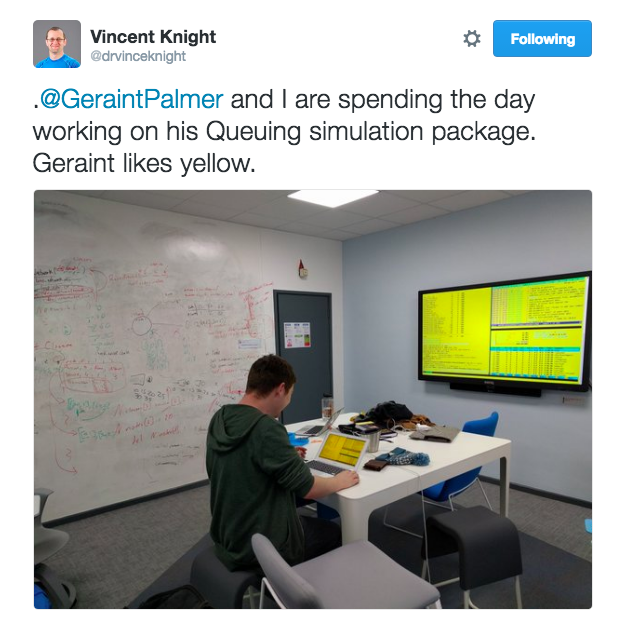
\includegraphics[width=0.7\textwidth]{tweets/sprinting_1}}
  \end{center}
\end{frame}

\begin{frame}
  \begin{center}
  \href{https://twitter.com/drvinceknight/status/732186687338651648}{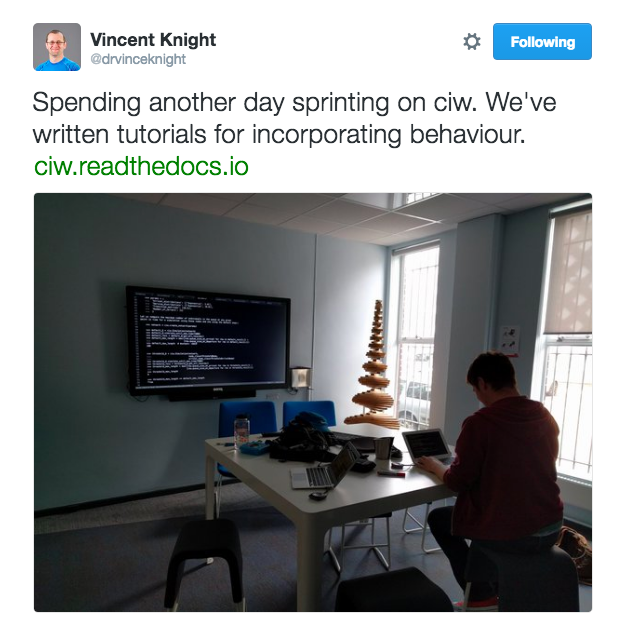
\includegraphics[width=0.7\textwidth]{tweets/sprinting_2}}
  \end{center}
\end{frame}

% Features - (Priority, baulking, preemptive interruptions)
\begin{frame}
  \begin{center}
  \href{https://twitter.com/CiwPython/status/748218828715360256}{
\includegraphics[width=0.9\textwidth]{tweets/priority_queues}}
  \end{center}
\end{frame}
\begin{frame}
  \begin{center}
  \href{https://twitter.com/CiwPython/status/750753028450443264}{
\includegraphics[width=0.9\textwidth]{tweets/baulking}}
  \end{center}
\end{frame}
\begin{frame}
  \begin{center}
  \href{https://twitter.com/CiwPython/status/780767974009430016}{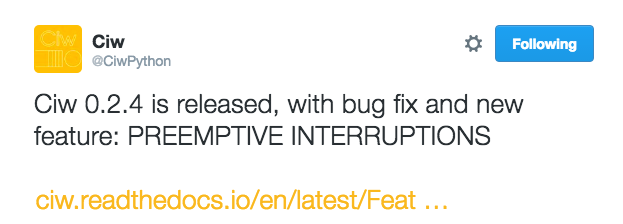
\includegraphics[width=0.9\textwidth]{tweets/preemptive_interruptions}}
  \end{center}
\end{frame}

% Communication - (Docs, PyCon UK, CORS, PyCon Namibia)
\begin{frame}
  \begin{center}
  \href{https://twitter.com/CiwPython/status/750697026023747584}{
\includegraphics[width=0.9\textwidth]{tweets/cymraeg_docs}}
  \end{center}
\end{frame}
\begin{frame}
  \begin{center}
  \href{https://twitter.com/GeraintPalmer/status/777931024336621568}{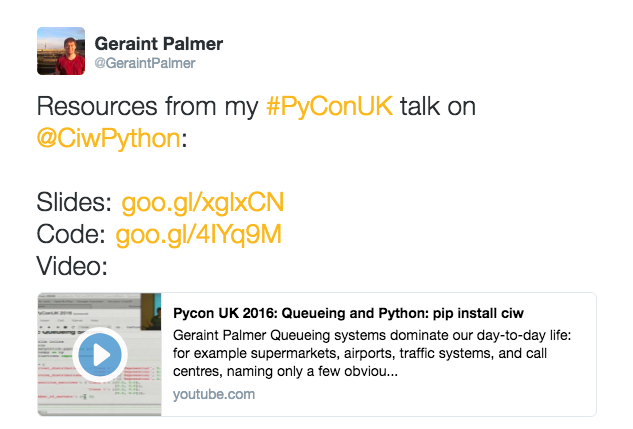
\includegraphics[width=0.9\textwidth]{tweets/pyconuk}}
  \end{center}
\end{frame}

\begin{frame}
  \begin{center}
  \href{https://twitter.com/profpaulharper/status/737411211063492608}{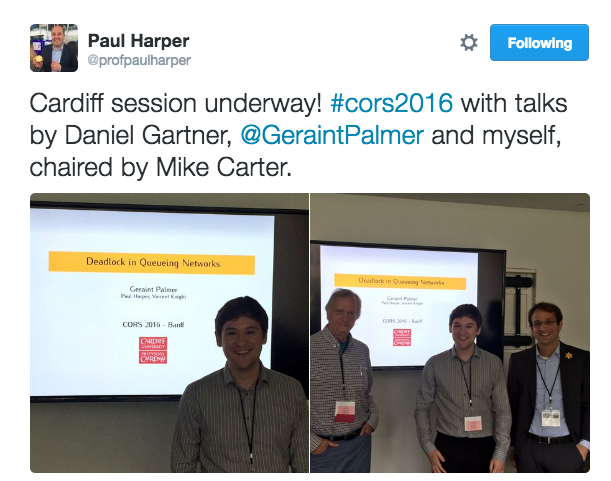
\includegraphics[width=0.8\textwidth]{tweets/cors}}
  \end{center}
\end{frame}

\begin{frame}
  \begin{center}
  \href{https://twitter.com/AishaXBello/status/692267117614362625}{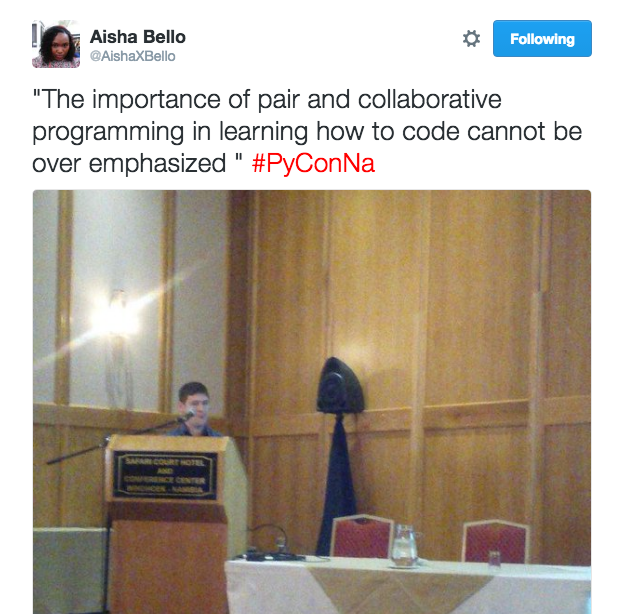
\includegraphics[width=0.7\textwidth]{tweets/pyconna_1}}
  \end{center}
\end{frame}

\begin{frame}
  \begin{center}
  \href{https://twitter.com/muheuenga/status/693380281340968960}{
\includegraphics[width=0.9\textwidth]{tweets/pyconna_3}}
  \end{center}
\end{frame}

% Uses - (Deadlock, Cindy, Jenny+Lieke (Errors))
\begin{frame}
  \begin{center}
  \href{https://twitter.com/GeraintPalmer/status/623530377932578816}{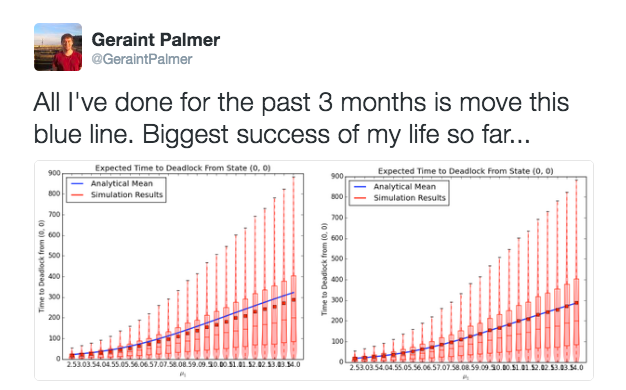
\includegraphics[width=0.9\textwidth]{tweets/deadlock_move_line}}
  \end{center}
\end{frame}

\begin{frame}
  \begin{center}
  \href{https://twitter.com/drvinceknight/status/766215470945009664}{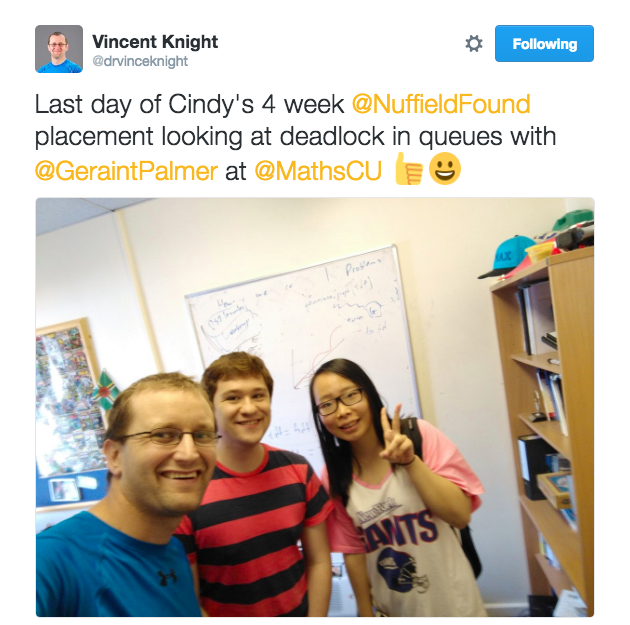
\includegraphics[width=0.7\textwidth]{tweets/nuffield_cindy}}
  \end{center}
\end{frame}

\begin{frame}
  \begin{center}
  \href{https://twitter.com/GeraintPalmer/status/710479754047197185}{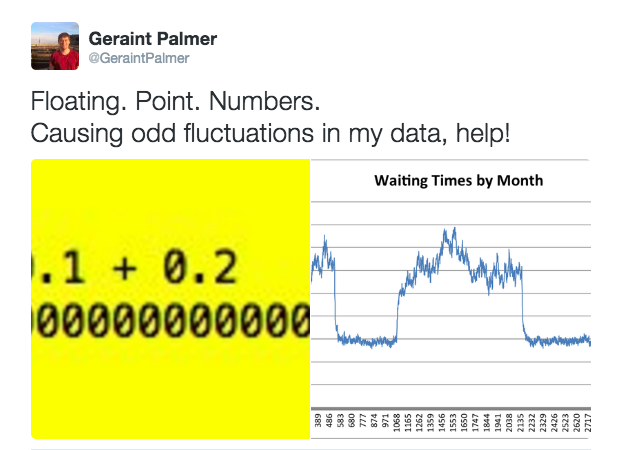
\includegraphics[width=0.9\textwidth]{tweets/floating_point_numbers}}
  \end{center}
\end{frame}

% CiwVis
\begin{frame}
  \begin{center}
  \href{https://twitter.com/CiwPython/status/765638369669939200}{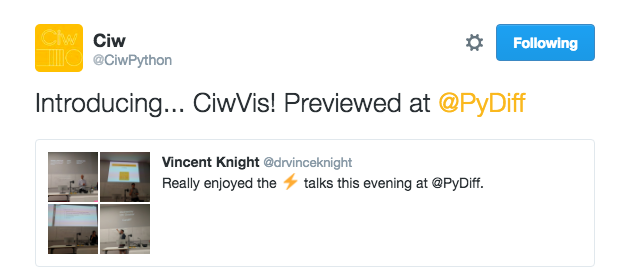
\includegraphics[width=0.9\textwidth]{tweets/ciwvis}}
  \end{center}
\end{frame}

% Animation
\begin{frame}
  \begin{center}
  \href{https://twitter.com/PyDiff/status/780692987038818304}{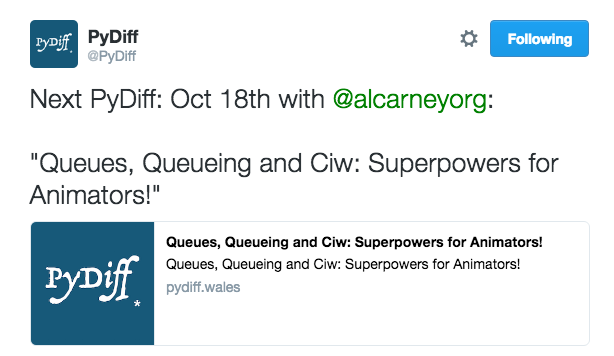
\includegraphics[width=0.9\textwidth]{tweets/animation_pydiff}}
  \end{center}
\end{frame}

% Follow Ciw
\begin{frame}
  \begin{center}
  \href{https://twitter.com/GeraintPalmer/status/747477836060049408}{
\includegraphics[width=0.9\textwidth]{tweets/follow_ciw}}
  \end{center}
\end{frame}

\end{document}
